%!TEX root = ../main.tex
\section{Experiment} 
\label{sec:exp}

\subsection{Experimental Settings}


\noindent \textbf{Our Experimental Scenario.} To demonstrate the performance of the \sys framework, we  analyze a simplified\footnote{why simplified?} real-world use case. The case compares  \sys framework with an open-source storage solution to build a big data processing pipeline that can facilitate business analysis. Specifically, a mobile financial application company collaborates with a mobile carrier to collect and analyze its app usage data. The company aims to understand its app usage patterns to prevent frauds and enhance its product experience. The mobile carrier provides this analytic service through an end-to-end big data processing pipeline. This pipeline includes several jobs such as data collection, normalization, labeling, and querying, as depicted in Figure~\ref{exp:fig:case}.

\noindent \underline{\textit{(a) Collection:}}  The network carrier collects mobile app data packets in  data centers across the nation via deep packet inspection (DPI) and transfers them to a centralized storage pool.

\noindent \underline{\textit{(b) Normalization:}} At the  storage pool, the data packets are normalized as records in a unified schema. Data is validated to ensure accuracy and quality. Sensitive data is shielded to protect  privacy. 

\noindent \underline{\textit{(c) Labeling:}} Labels from knowledge bases are added, so as to classify the records and identify useful insights.

\noindent \underline{\textit{(d) Query:}} After the normalization and labeling processes are completed, the  records are inserted into tables and are available for query engines. To perform analyses, the app company employs secure API calls to query the data. Figure~\ref{exp:fig:sql} illustrates an example SQL query that counts the daily active users (DAU) in different provinces. More complicated analysis, like hidden Markov and Gaussian Mixture Models\footnote{why mention models?}, can also be applied to draw user profiles and identify abnormal activities.

To support both full data and real time analyses, the network carrier builds two data flows in the pipeline. One flow processes full data in batch every two hours and the other processes stream messages constantly to deliver time-sensitive logs such as new logins, payments and password modifications. This ensures that the network carrier can effectively analyze both historical data and real-time events to make  accurate and timely decisions.

 \begin{figure}[htbp]
	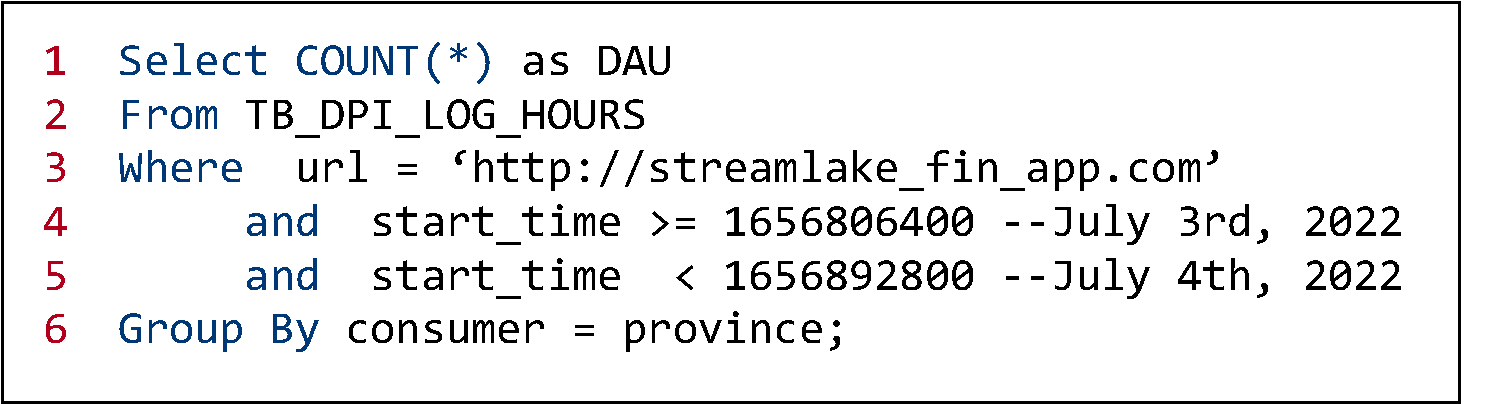
\includegraphics[scale=0.35]{figures/sql}
	\centering
	\vspace{-1em}
	\caption{Query Example of Computing DAU.}
	\label{exp:fig:sql}
\end{figure}

\noindent \textbf{Settings.} This use case is evaluated in a commodity\footnote{@} cluster using different sizes of input data packets and the results are compared with open-source storage solution Hadoop Distributed File System (\hdfs)~\cite{} and \kafka~\cite{}. The reason of why we choose the two storage systems is that in reality, China Mobile has been using them for many years, which have shown stable and good performance. Hence, it is  reasonable to directly compare with the systems that our customer (China Mobile) is using. Also, in practice, as we know, many other companies also use HDFS and Kafka to cope with similar application scenarios.
\cc{For above, do we need more justification? like why hdfs and kafka fit? or common sense?}
%These two storage systems are chosen because of their popularity in real world and are relatively easy to provide context to illustrate the usage of StreamLake.


 
  To be specific, the cluster hardware\footnote{cluster hardware?}  consists of 3 nodes, each with 24  2.30 GHz cores and 256 GB RAM. The cluster is configured as a 3-node \sys when we measure it.  While running the open-source solution, it is configured to host a 3-node \hdfs storage and a 3-node \kafka cluster simultaneously. The number of input data packets varies: 10 million, 50 million, 100 million, 500 million, and 1 billion packets. Each packet has an average size of 1.2 KB, resulting in corresponding data volumes of 12 GB, 60 GB, 120 GB, 600 GB, and 1.2 TB, respectively.

Overall, Figure~\ref{exp:fig:case} shows the data processing process.  \kafka and \hdfs serves as independent stream storage and batch storage respectively to pass data across collection, normalization, labeling and query jobs.
 As a typical ETL practice, a new copy of all data is written to \hdfs and \kafka after each job. In case it\footnote{who?} fails accidentally, a job can read its input data to reproduce the results.
 
 
 \begin{figure*}[htbp]
 	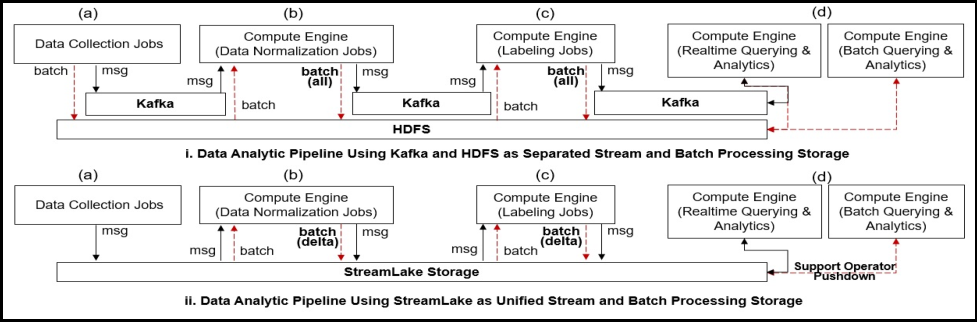
\includegraphics[scale=1.05]{figures/case}
 	\centering
 	\vspace{-1em}
 	\caption{Data Analytic Pipelines for a  Real-world Use Case.}
 	\label{exp:fig:case}
 \end{figure*}
 
  In our solution, \sys serves as a unified stream and batch processing storage. \cc{It reads messages from the data collection jobs and passes messages and aggregated batches to the same stream and batch processing engines in the normalization, labeling and query jobs.}\footnote{too many and} 
  As \sys supports time travel, only updated rows are written to the storage. When a job needs to re-run, it can use time travel to retrieve its input data.  During the query jobs, for example, the three filters in the \texttt{WHERE} clause and the \texttt{COUNT} aggregate in Figure~\ref{exp:fig:sql} are pushed down to compute in \sys, so as to  accelerate the query.


\begin{table*}[ht]
	\begin{tabular}{|c|c|c|c|c|c|c|}
		\hline
		&  \#-Data Packet & 10,000,000 & 50,000,000 & 100,000,000 & 500,000,000 & 1,000,000,000 \\ \hline
		\multirow{3}{*}{Storage Space Usage (GB)}                  & \sys              & 34         & 166        & 329         & 1,659       & 3,289         \\ \cline{2-7} 
		& \hdfs + \kafka            & 145        & 729        & 1451        & 6,901       & 13,816        \\ \cline{2-7} 
		& Ratio (HK/S)         & 4.33       & 4.38       & 4.40        & 4.16        & 4.20          \\ \hline
		\multirow{3}{*}{Stream Processing Speed (Messages/Second)} & \sys              & 301,522    & 417,303    & 518,065     & 530,077     & 546,987       \\ \cline{2-7} 
		& \kafka             & 302,611    & 413,613    & 527,826     & 531,021     & 539,893       \\ \cline{2-7} 
		& Ratio (K/S)         & 1.00       & 0.99       & 1.02        & 1.00        & 0.99          \\ \hline
		\multirow{3}{*}{Batch Processing Total Time (Second)}      & \sys             & 259        & 664        & 1173        & 4868        & 9646          \\ \cline{2-7} 
		& \hdfs              & 212        & 795        & 1548        & 7535        & 14771         \\ \cline{2-7} 
		& Ratio (H/S)         & 0.82       & 1.19       & 1.32        & 1.55        & 1.53          \\ \hline
	\end{tabular}
\caption{\sys v.s. \hdfs and \kafka.}\label{tab:case}
\end{table*}


\subsection{Overall Comparison}

Table~\ref{tab:case} shows the results. The numbers of input data packets are in the top row. The storage usage and processing time for \sys (S), \hdfs (H), \kafka (K) are in the following rows.  The ``Ratio'' represents that the ratio between \hdfs(\kafka) and \sys with respect to the storage usage or time. 
Note that HK denotes the sum of the storage usage in  \hdfs and \kafka.

The experiment demonstrates that \sys significantly improves the total storage usage and the batch processing time. The storage usage in the \hdfs and \kafka  is 4 times as much as \sys. The reason is that in \hdfs and \kafka, full data is written into the storage when each ETL job is finished, which is a common practice to support downstream jobs restart after unexpected failures. As a result, six copies of full data are written into the storage. While for our \sys, since the storage natively supports time travel, we only save one copy of full data plus updates in each ETL job, saving about 75\% storage usage.


The batch processing speed in \sys is better than \hdfs when the workload is 50 million records or more.  As the workload grows, the advantage of skipping irrelevant partitions becomes significant. \sys is 50\% faster than \hdfs when the workloads are 500 million and 1 billion records. On the other hand, \sys may not be the best choice for small workloads. When the workload is 10 million records, \sys is 20\% slower than \hdfs as it performs extra metadata management.

\cc{Why not remove the first column??}



\cc{For the above, can we correspond to the designs with respect to previous sections as the reasons of improvement}

The message stream processing speed in \sys is competitive to \kafka. \sys and \kafka process about 300 thousand messages per second when the workload is 10 million records. Both systems scale to process about 500 thousand messages per second when the workloads are 100 million and more. 


\subsection{Evaluation of Message Streaming}


\subsection{Evaluation of LakeBrain}

\subsection{Evaluation of Query Pushdown}


\subsection{China Mobile Use Case}